\exrc (4 points) Effectuer les calculs suivants

\begin{tabularx}{\textwidth}{Y|Y}
    \cnt  & \cnt  \\
    $3+5\times 7 -3+1$ & $4+5\times (6-3+2)$
\end{tabularx} 

\exrc (2 points) Compléter le tableau suivant \textbf{(peut être fait sur le sujet)}.

\begin{tabularx}{\textwidth}{Y|Y}
    Forme décimale & Forme pourcentage \\ \hline
    & 35\% \\ \hline
    0,65 & \\ \hline
    & 9\% \\ \hline
    0,8 & 
\end{tabularx} 

\exrc (4 points) A l'aide du diagrame ci dessous.

\begin{figure}[H]
    \centering
    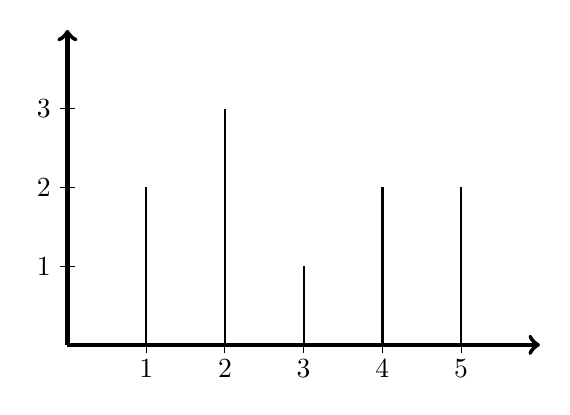
\begin{tikzpicture}
    \draw[ultra thick,->] (0,0)--(6,0) ; 
    \draw[ultra thick,->] (0,0) -- (0,4) ; 
    \foreach \r in {1,...,5}{\draw[color=black] (\r , -0.1)--(\r , 0.1);
    \draw (\r , -0.3) node {\r} ;}
    \foreach \r in {1,...,3}{\draw[color=black] (-0.1,\r )--( 0.1, \r);
    \draw (-0.3 , \r) node {\r} ;}
    \draw[thick] (1,0) -- (1,2) ;
    \draw[thick] (2,0) -- (2,3) ;
    \draw[thick] (3,0) -- (3,1) ;
    \draw[thick] (4,0) -- (4,2) ;
    \draw[thick] (5,0) -- (5,2) ;
    \end{tikzpicture}
    \end{figure}

\cnt (2 points) Compléter le tableau d'effectif \textbf{(peut être fait sur le sujet)}.

\begin{tabularx}{\textwidth}{Y*{5}{|Y}}
    Valeur &  1 & 2 & 3 & 4 & 5\\ \hline
    Effectif &  &  &  & &
\end{tabularx} 

\cnt (1 point) Calculer la fréquence de la valeur 5.

\cnt (1 point) Calculer la fréquence de la valeur 3.

\newpage

\exrc (5 points) Calculer les moyennes des séries suivantes

\cnt (2 points) 1 ; 2 ; 3 ; 4 ; 10 

\cnt (2 points) 5 ; 11 ; 14 ; 8 ; 13 ; 9

\cnt (1 points) la série définie par le tableau suivant :

\begin{tabularx}{\textwidth}{Y*{4}{|Y}}
    Valeur &  2 & 4 & 5 & 10\\ \hline
    Effectif & 3 & 1 & 2 & 4
\end{tabularx} 

\exrc (5 points) Calculer les médianes des séries suivantes

\cnt (2 points) 1 ; 2 ; 3 ; 4 ; 5 

\cnt (2 points) 12 ; 13 ; 7 ; 5 ; 1 ; 2

\cnt (1 points) la série définie par le tableau suivant :

\begin{tabularx}{\textwidth}{Y*{5}{|Y}}
    Valeur &  12 & 15  & 19 & 25 & 39\\ \hline
    Effectif & 2 & 1 & 1 & 4 & 3
\end{tabularx} 